\documentclass[10pt]{article}

\usepackage{amsthm, amsmath, amsfonts, cancel, pdfpages, float}
\newcommand{\Z}{\mathbb{Z}}
\newcommand{\R}{\mathbb{R}}
\newcommand{\N}{\mathbb{N}}
\graphicspath{ {../screenshots/} }

\begin{document}

\date{02/25/19}


\title{HomeWork 4}
\author{Chris Humphreys \& Adam Chisholm\\ 
CS455 - Data Mining\\University of Tennessee at Martin } 

\maketitle
\section*{1.}
In the below screenshots, you can see our inital setup and usage of R.   See 
figure \ref{fig:r1} for initial setup.   See figure \ref{fig:r2} for the 
histogram of the Sepal Lengths. 
\begin{figure}[]
    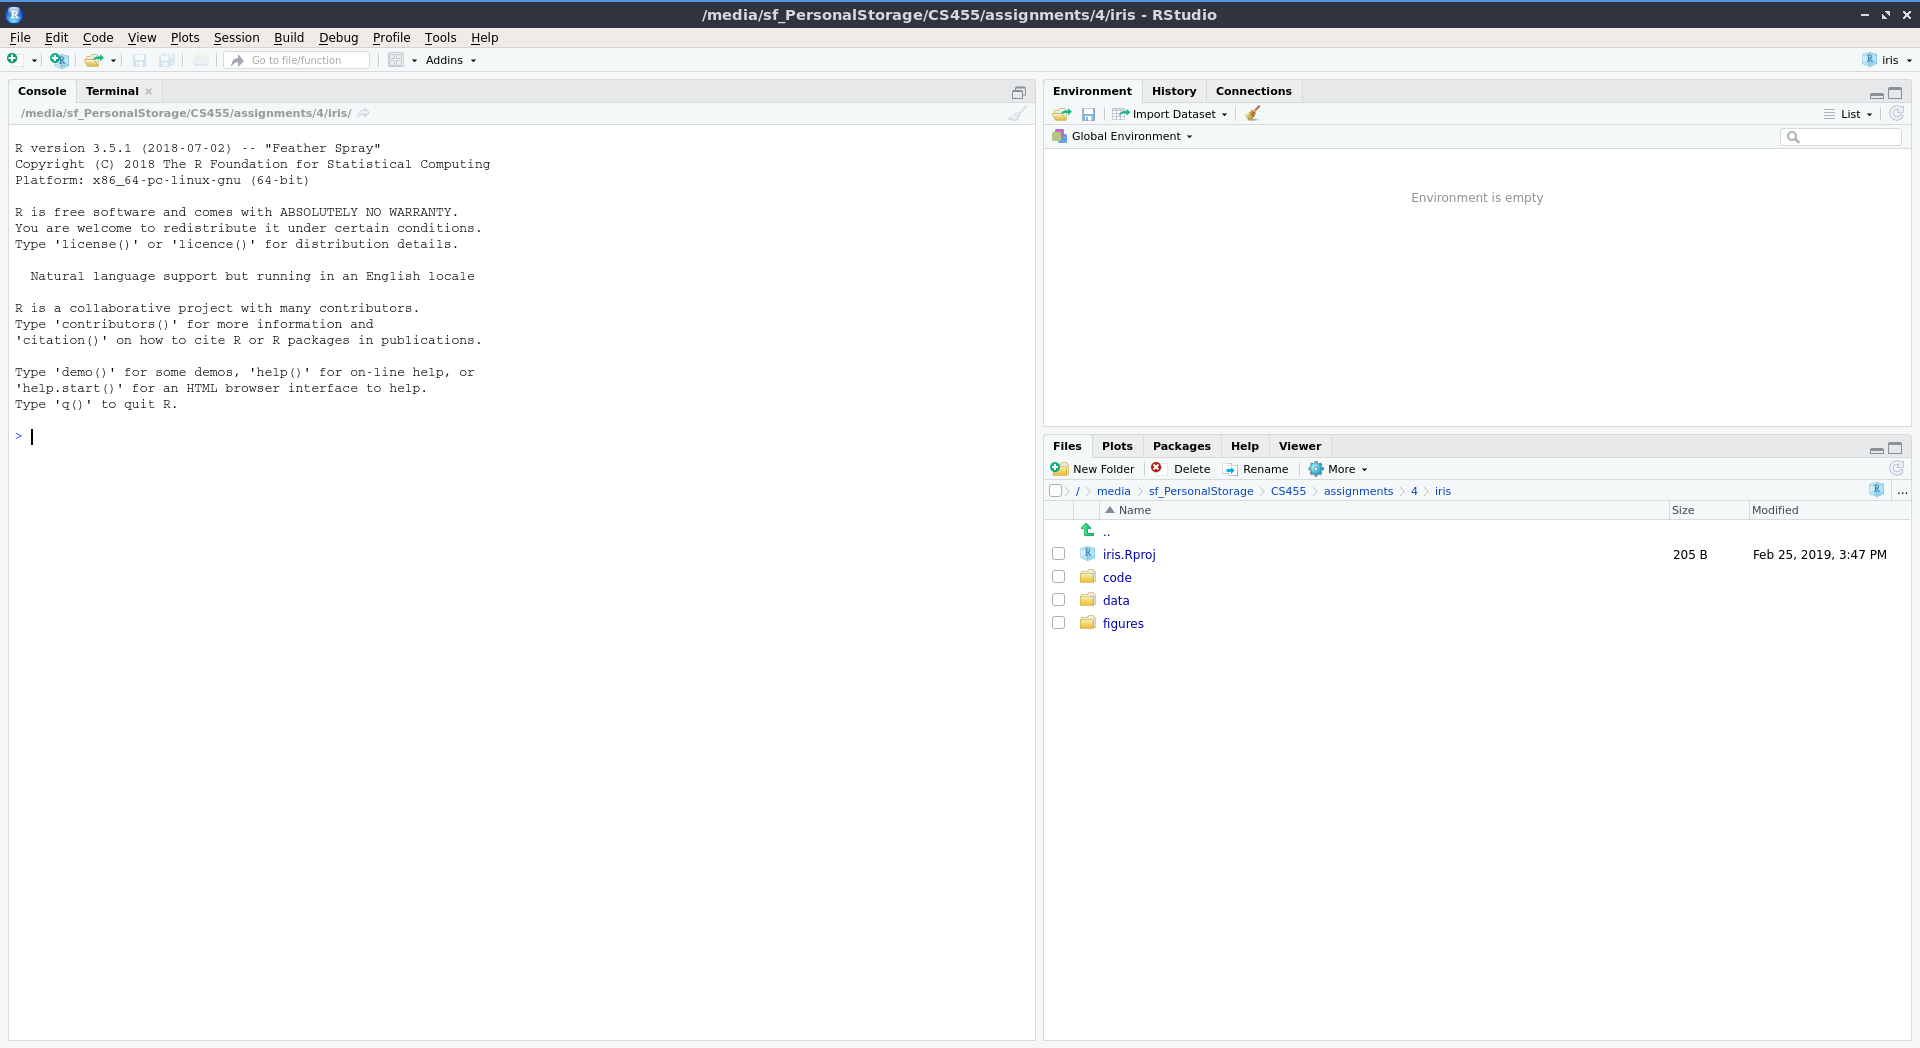
\includegraphics[width=\textwidth]{initSetup}
    \caption{Initial setup of R}
    \label{fig:r1}
\end{figure}
\begin{figure}[]
    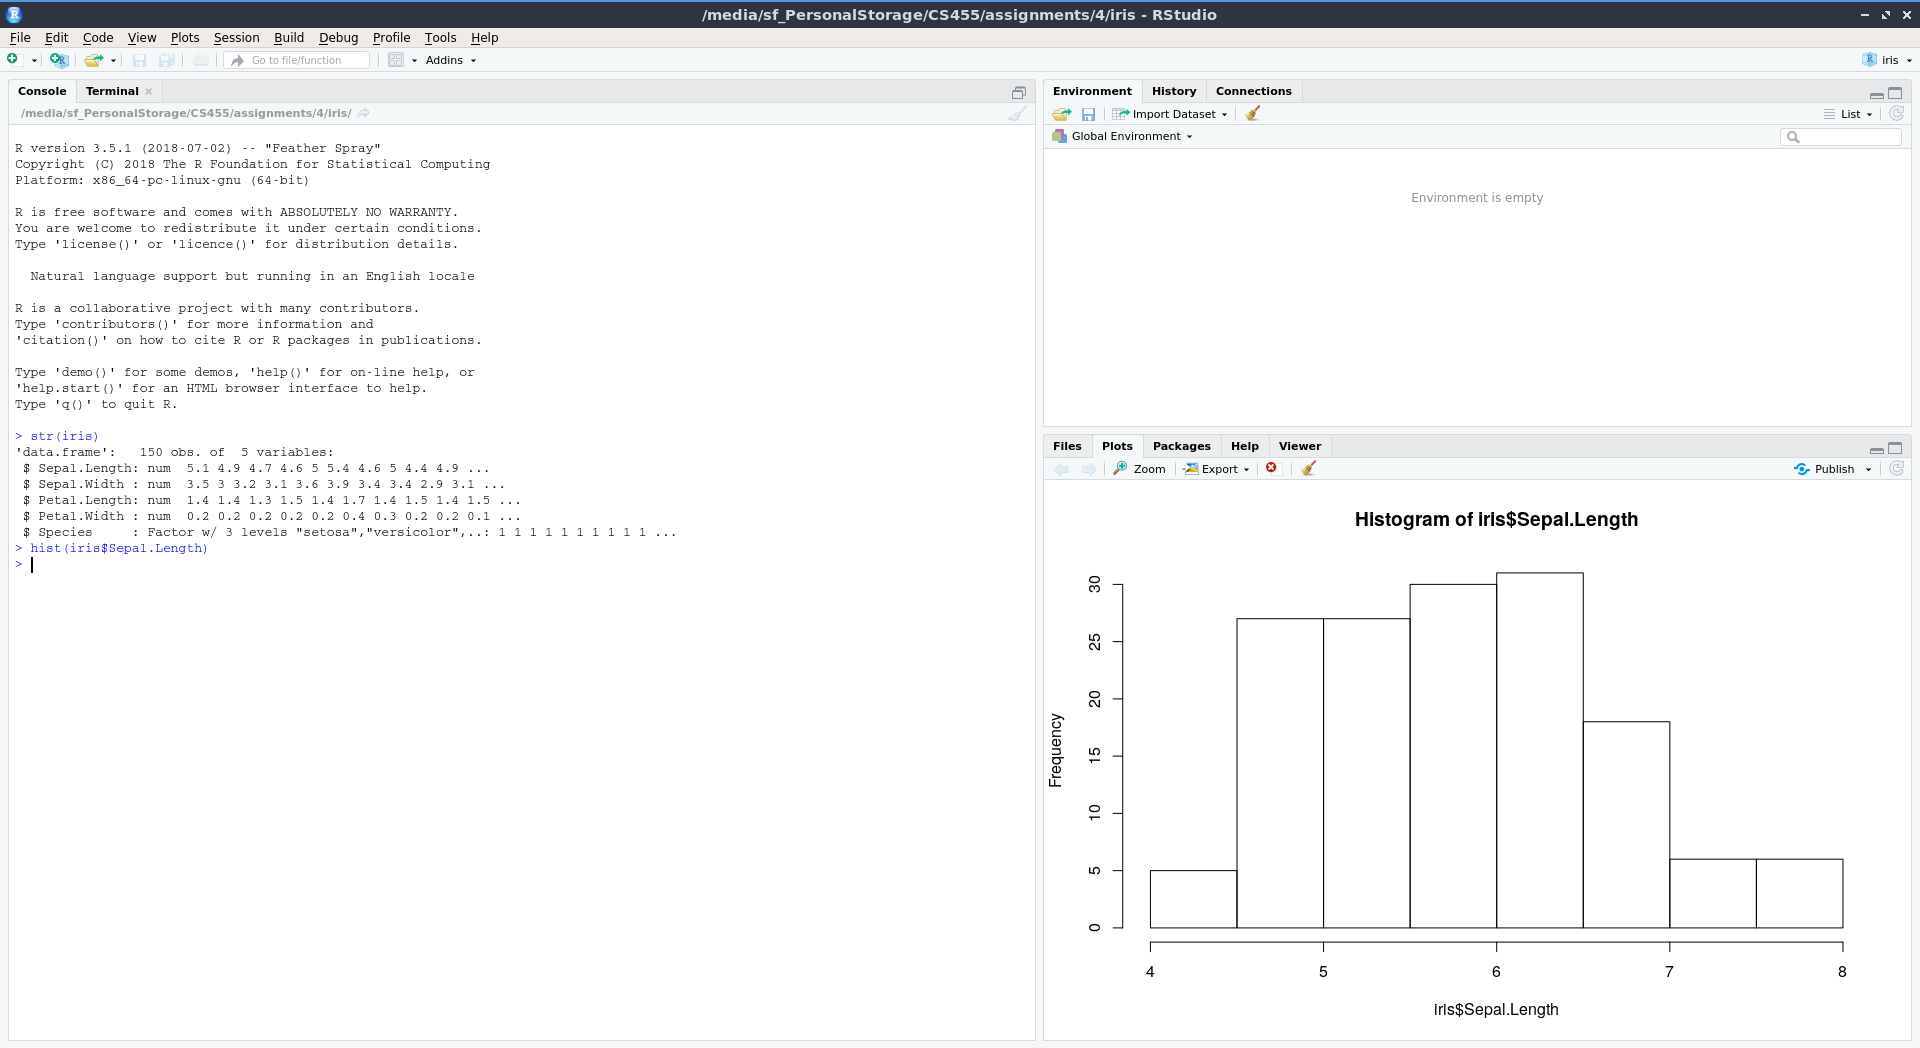
\includegraphics[width=\textwidth]{irisHist}
    \caption{Iris historgram in RStudio}
    \label{fig:r2}
\end{figure}
\section*{2.}
Figure \ref{fig:weka1} is a screenshot of our initial setup of Weka.  In this 
screenshot we have created the histogram for the sepal length, but have not 
applied any filters to it.  You will notice that the histograms in figure 
\ref{fig:r2} and figure \ref{fig:weka1} are different although they come from 
the same data set.  This is due to the fact that in RStudio (figure 
\ref{fig:r2}) the histogram starts at 4 and ends at 8, and is composed of 8 
bins, each 1/2 cm wide, while in Weka (figure \ref{fig:weka1}) the bins start at 
the minimum sepal length of 4.3 and go up to the maximum sepal length of 7.9.  
Additionally, the Weka histogram is composed of only 7 bins that are a bit over
.5 cm each.  
\begin{figure}[]
    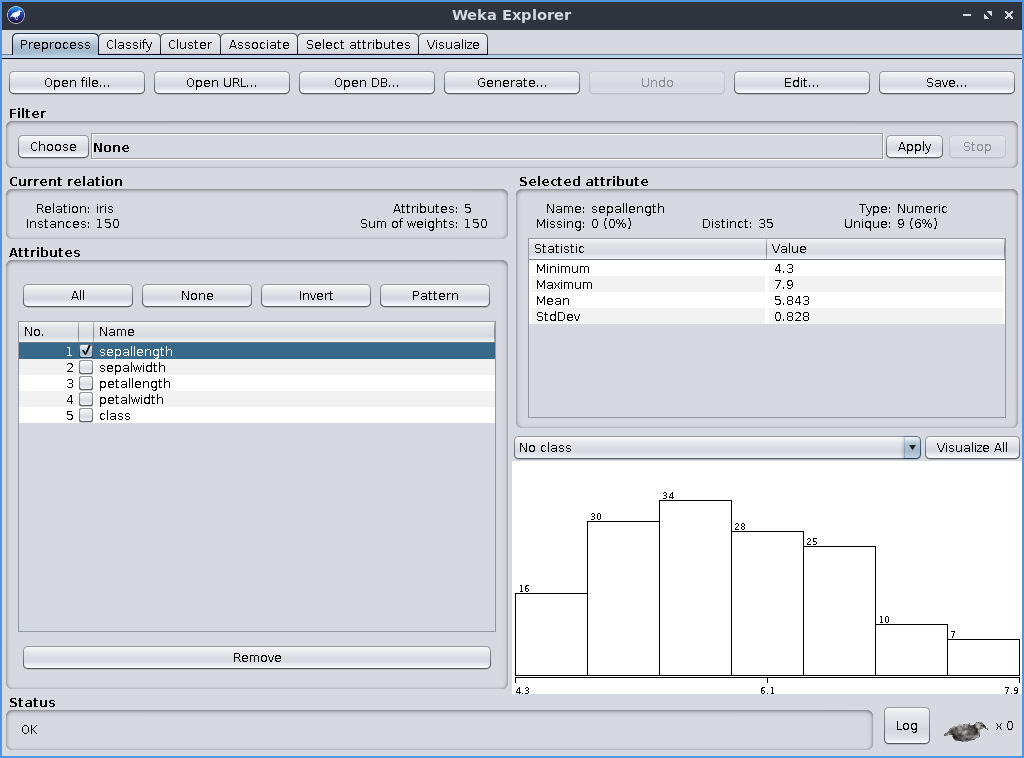
\includegraphics[width=\textwidth]{selectWeka}
    \caption{Iris histogram in Weka, no filters}
    \label{fig:weka1}
\end{figure}
\section*{3.}
Figure \ref{fig:weka2} shows the same sepal data again, but this time after
being filtered as directed in the assignment in question 3.  This time the 
histogram still looks different than the histogram in figure \ref{fig:r2}.
There are a number of reasons for the two histograms looking different.  First 
is the fact that although we have 8 bins in both, the first bin in figure 
\ref{fig:r2} contains all the sepal lengths from 0 to 4.5, while the first bin
in figure \ref{fig:weka2} contains all the sepal lengths from 0 to 4.75.  From 
these different starting points of 4.5, and 4.75, figure \ref{fig:r2} creates a
new bin every .5 cm, while figure \ref{fig:weka2} creates a new bin every .45 
cm. This difference does not seem like much initially, but as can be seen in the 
figures below, it can result in a significant difference in the final histogram.
\begin{figure}[]
    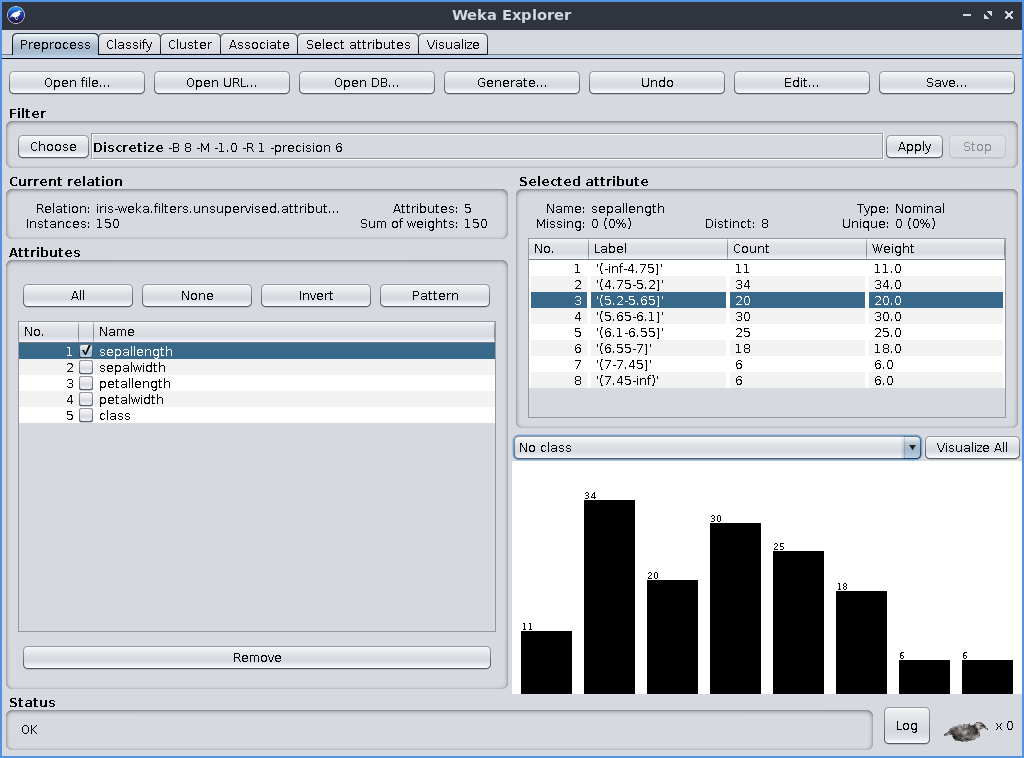
\includegraphics[width=\textwidth]{wekaFiltered}
    \caption{Iris histogram in Weka with filters}
    \label{fig:weka2}
\end{figure}
\end{document}
